\section{Implementation results}

\begin{frame}{Software ecosystem}
    \begin{tikzpicture}[node distance = 1cm, auto]

	\node [whtblock,text depth=14mm] (FEDDLIB) {
		{\footnotesize \textbf{FEDDLib}\textsuperscript{a}} \\[0.3em] \tiny \textbf{F}inite \textbf{E}lement and \textbf{D}omain \textbf{D}ecomposition \textbf{Lib}rary
		\begin{itemize}
			\item{Parallel finite element assembly}
			\item{Specific problem definition}
			\item{Mesh handling routines}
			      % \item \textcolor{orange}{Update two-level nonlinear Schwarz solver for elasticity and Navier-Stokes}
			      % \item \textcolor{orange}{Test with various coarse spaces}
		\end{itemize}
		% \hspace*{-25mm}\scalebox{.7}{By University of Cologne, TU Delft, TU Freiberg}
	};

	\node [whtblock, right=of FEDDLIB,node distance=7cm, rectangle split part fill={orange!20,blue!5},] (FeatFlow) {
		{ \footnotesize\textbf{FEAT3}\textsuperscript{b}}\\[0.3em] \tiny Finite element based solution of incompressible\\Navier-Stokes in 2D and 3D
		\vspace{2pt}
		\begin{itemize}
			%\setlength{\itemsep}{0pt}
			\item \textcolor{red}{Interface with \texttt{FROSch}}
			\item \textcolor{red}{Test (non-Newtonian, high Reynolds, exascale)}
		\end{itemize}};

	%===============================================    
	\node [whtblock, below=of FEDDLIB, text depth=18mm, node distance=3.5cm,] (Trilinos) {
		{\footnotesize \textbf{Trilinos}\textsuperscript{c}}
		\begingroup
		\addtolength{\leftmargini}{0.5cm}
		\vspace{1pt}
		\tiny
		\begin{itemize}
			%\setlength{\itemsep}{0pt}
			\item Data services: Vectors, matrices, graphs and related operations
			\item Linear and Eigenproblem solvers
			\item Nonlinear solvers and analysis tools
		\end{itemize}
		\endgroup
	};

	\node[inner sep=0pt] (trilinos_logo) at ([xshift=6mm, yshift=0mm] Trilinos.west){
\includegraphics[width=.125\textwidth, angle=90,origin=c]{images/logo/Trilinos_logo_new.png}};

	\node [whtblock, text depth=18mm, right=of Trilinos,node distance=7cm,rectangle split part fill={orange!20,blue!5},] (Frosch) {
		{\footnotesize \textbf{FROSch}\textsuperscript{d}} \\[0.4em]  \hspace{6em}\tiny\textbf{F}ast and \textbf{R}obust \textbf{O}verlapping \textbf{S}chwarz
		\vspace*{0.5em}
		\begingroup
		\addtolength{\leftmargini}{4em}
		\begin{itemize}
			\item \textcolor{red}{Implement two-level nonlinear Schwarz solver}
			\item \textcolor{red}{Test with various coarse spaces on various model problems}
		\end{itemize}
		\endgroup
	};

	\node[inner sep=0pt] (trilinos_logo) at ([xshift=7.5mm, yshift=0mm] Frosch.west){
\includegraphics[width=.1\textwidth]{images/logo/FROSch_logo.png}};

	%%%%%%%%%%%%%%%%%%%%%%%%%%%%%%%%
	%   CONTAINERS -- BACKGROUND LIGHT-DASHED BLOCKS
	%%%%%%%%%%%%%%%%%%%%%%%%%%%%%%%%
	\begin{scope}[on background layer]

		\coordinate (aux2) at ([yshift=0mm]Trilinos.north);
		\node[container2, fit=(aux2) (Trilinos) (Frosch)] (Trilinos_blue) {};

		\coordinate (aux3) at ([yshift=0mm] FeatFlow.north);
		\node[container3, fit=(aux3) (FeatFlow)] (FeatFlow_Green) {};

		\coordinate (aux1) at ([yshift=0mm]FEDDLIB.north);
		\node [container,fit=(aux1) (FEDDLIB)] (FEDDLIB_ORANGE) {};
		\node at ([yshift=0.7mm]Trilinos_blue.north) [fill=gray!10,draw,minimum width=8em,minimum height=1em] (FEDTRI-label) {\footnotesize\textbf{Interface}};

	\end{scope}
	%************************************************************
	%************************************************************
	%  Draw edges
	%************************************************************
	%************************************************************
	% \path [line,thick] (FEDDLIB) -- (FEDTRI-label);
	% \path [line,thick] (Trilinos) -- (Frosch);
	% \path [line,thick] (FEDTRI-label) -- (Trilinos);
	% \path [line,red,thick] (FeatFlow) -- (FEDTRI-label);

\end{tikzpicture}
\tiny\\~\\

a: University of Cologne, TU Delft, TU Freiberg (https://github.com/FEDDLib/FEDDLib.git)\\
b: TU Dortmund (https://github.com/tudo-math-ls3/feat3)\\
c: Sandia National Laboratories (https://trilinos.github.io)\\
d: University of Cologne, TU Delft, TU Freiberg (https://shylu-frosch.github.io)\\

\end{frame}
\subsection{Neo-Hookean hyperelasticity}

\begin{frame}{2D compressible plane-stress neo-Hookean material}
	\vspace{0mm}
	\begin{columns}
		\begin{column}{0.4\textwidth}%
			\begin{align*}
				\label{eq:nonlinelas}
				\begin{split}
					-\mathrm{div}(P(F)) = f_{vol}\; & \mathrm{in}\;\Omega,           \\
					u = g_D \;                      & \mathrm{on}\;\partial\Omega_D, \\
					n\cdot P(F) = g_N\;             & \mathrm{on}\;\partial\Omega_N,
				\end{split}
			\end{align*}
			\begin{figure}
				\centering
				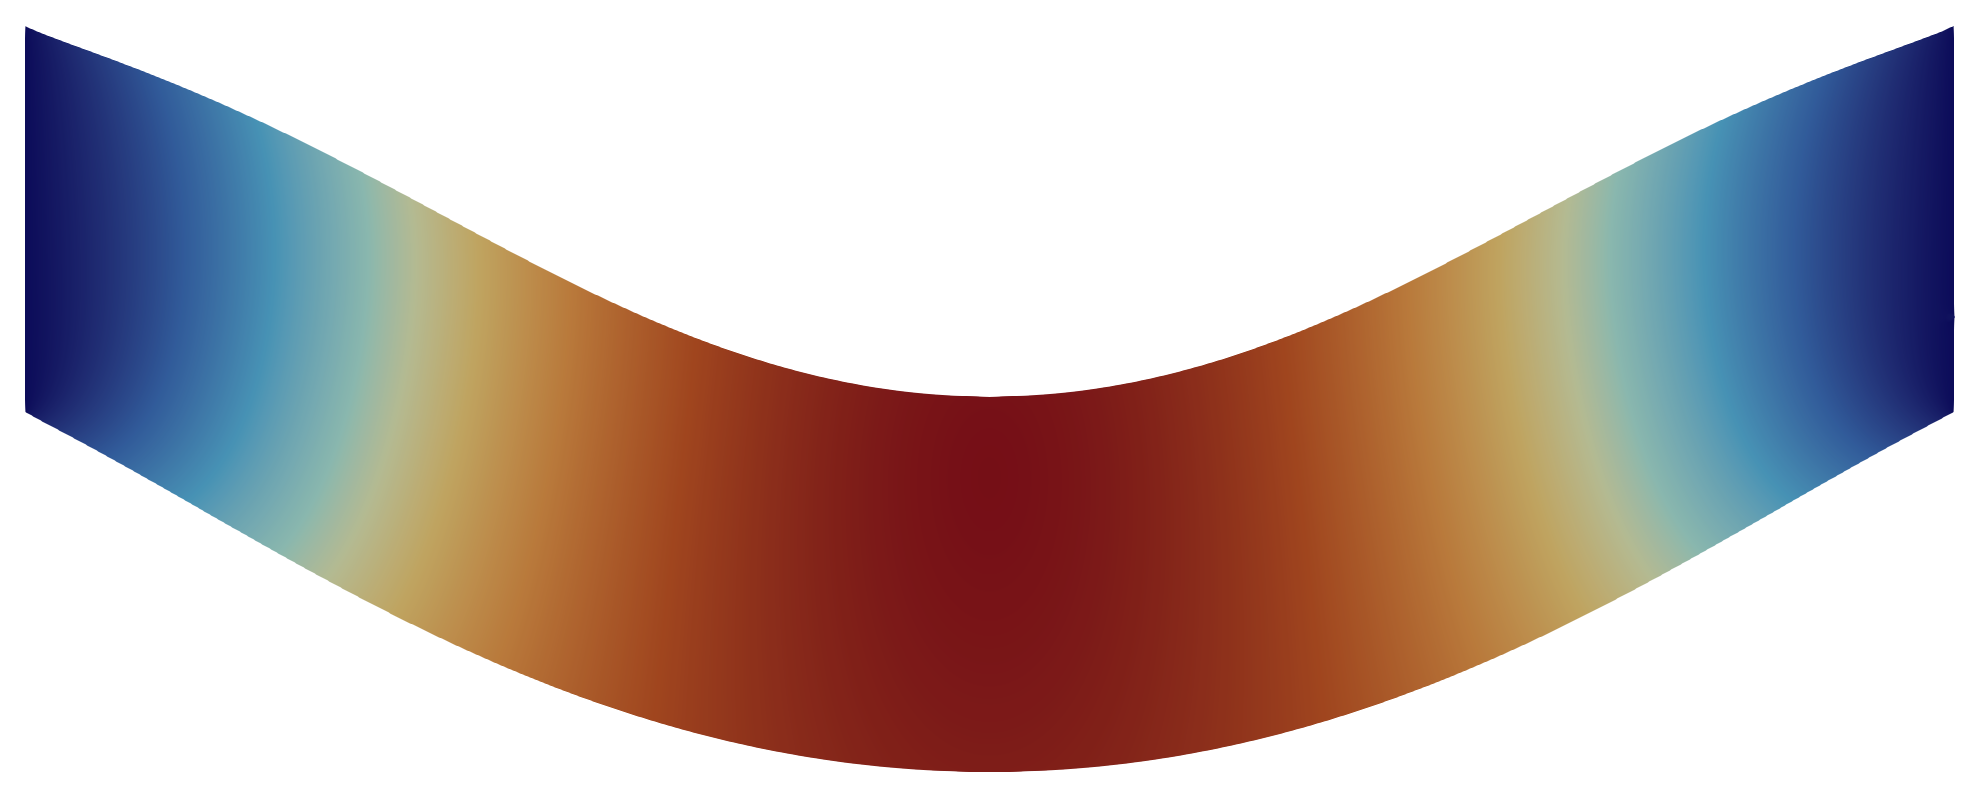
\includegraphics[width=0.9\textwidth]{images/beam2D.png}
				\caption{2D beam with applied volume force.}
				\label{fig:beam2d}
			\end{figure}
		\end{column}%
		\begin{column}{0.6\textwidth}
			\vspace{-1em}
			\centering
			\begin{itemize}
				% \setlength{\itemsep}{15pt}
				\item $F$ Deformation gradient
				\item $P(F) = \frac{E}{1(1+\nu)}(F-F^{-T}) + \frac{E\nu}{(1+\nu)(1-2\nu)}\mathrm{ln}(\mathrm{det}(F)F^{-T})$
				\item $\nu$ = 0.3
				\item $E$ = 210 GPa
				\item $5\textrm{m}\times 1\textrm{m}$ 2D mesh with \numgru{2572710} nodes
        \item $g_D = 0$ on short edges
				\item $g_N = 0$ on long edges
				\item P1 elements
        \item Solver relative tolerance: $10^{-4}$
        \item MsFEM coarse space \footnotemark{}
				% \item $f_{vol} = (0,-f_y)$
			\end{itemize}
		\end{column}
	\end{columns}
  \footnotetext{\tiny Dohrmann, Widlund (2017)}
\end{frame}

\begin{frame}{Strong scaling: nonlinear elasticity}
	\begin{itemize}
		\item $f_y = 4$ MN/m$^{2}$
	\end{itemize}
	\begin{figure}
		\centering
		\begin{tikzpicture}
	\pgfplotsset{
		every axis/.append style={
				ybar stacked,
				width=13cm,
				height=7cm,
				ylabel={Runtime (seconds)},
				xlabel={Num. subdomains},
				symbolic x coords={72, 144, 288, 576, 1152},
				xtick=data,
				enlarge x limits=0.15,
				legend style={at={(1,1)},anchor=north east},
				axis lines*=left, ymajorgrids, yminorgrids,
				ymin=0,
				ymax=100,
				bar width=8pt,
				minor y tick num=1,
				xticklabel style={rotate=0,xshift=0ex,anchor=north},
				cycle list name=Set2-5,
			},
		% Ensures that bars are plotted full
		every axis plot/.append style={
				fill,
			},
	}
	\tikzstyle{mynodestyle} = [rotate=90, anchor=west]

	% Solver = H1
	\begin{axis}[bar shift=11pt, hide axis]
		% Another option for relative node placement
		% \node [left=11pt of 256.base, anchor=base] {test}; % Custom number above bar for 256
		\node[mynodestyle] at ([xshift=11pt]axis cs:72,58) {$65$ $(3)$};
		\node[mynodestyle] (one) at ([xshift=11pt]axis cs:144,27.5) {$62$ $(3)$};
		\node[mynodestyle] at ([xshift=11pt]axis cs:288,13.6){$53$ $(3)$};
		\node[mynodestyle] at ([xshift=11pt]axis cs:576,6.8){$44$ $(3)$};
		\node[mynodestyle] at ([xshift=11pt]axis cs:1152,4.5){$41$ $(3)$};
		\node [mynodestyle](oneRe) at ([xshift=11pt]axis cs:72,1) {H};

		\addplot coordinates {(72,58) (144,27.5) (288,13.6) (576,6.8) (1152,4.5)};
	\end{axis}

	% Solver = Add.
	\begin{axis}[bar shift=0pt, hide axis]
		\node[mynodestyle] at (axis cs:72,81.2) {$100$ $(4)$};
		\node[mynodestyle](two) at (axis cs:144,34.5) {$97$ $(4)$};
		\node[mynodestyle]at (axis cs:288,17) {$81$ $(4)$};
		\node[mynodestyle]at (axis cs:576,9) {$75$ $(4)$};
		\node[mynodestyle]at (axis cs:1152,6.2) {$71$ $(4)$};
		\node [mynodestyle]at (axis cs:72,1) {Add.};

		\addplot+ coordinates {(72,81.2) (144,34.5) (288,16.9) (576,9) (1152,6.2)};
	\end{axis}

	% Solver = NKS

	\begin{axis}[bar shift=-11pt]
		%% Overlap = 10
		% \node [mynodestyle] at([xshift=-11pt]axis cs:72,42) {$190$ $(5)$};
		% \node [mynodestyle](three) at([xshift=-11pt]axis cs:144,22.5) {$200$ $(5)$};
		% \node [mynodestyle]at([xshift=-11pt]axis cs:288,11.8) {$170$ $(5)$};
		% \node [mynodestyle]at([xshift=-11pt]axis cs:576,7.3) {$150$ $(5)$};
		% \node [mynodestyle]at([xshift=-11pt]axis cs:1152,5.2) {$135$ $(5)$};
		% \node [mynodestyle]at ([xshift=-11pt]axis cs:72,1) {NKS};
		%
		% \addplot+ coordinates {(72,41.7) (144,22.5) (288,11.8) (576,7.3) (1152,5.2)};


		%% Overlap = 5
		\node [mynodestyle]at([xshift=-11pt]axis cs:72,33) {$162$ $(5)$};
		\node [mynodestyle](three) at([xshift=-11pt]axis cs:144,16) {$159$ $(5)$};
		\node [mynodestyle]at([xshift=-11pt]axis cs:288,8) {$136$ $(5)$};
		\node [mynodestyle]at([xshift=-11pt]axis cs:576,4) {$124$ $(5)$};
		\node [mynodestyle]at([xshift=-11pt]axis cs:1152,3.2) {$108$ $(5)$};
		\node [mynodestyle]at([xshift=-11pt]axis cs:72,1) {NKS};

		\addplot+ coordinates {(72,34) (144,17.1) (288,9.1) (576,5.1) (1152,4.2)};
		\node[text width=1.6cm] (gmres) at (axis cs:144,80){GMRES its. (Newton its.)};

	\end{axis}

	\draw [thin] (gmres) --  (one);
	\draw [thin] (gmres) --  (two);
	\draw [thin] (gmres) --  (three);

\end{tikzpicture}

		\label{fig:strong-scalability-elascticity}
	\end{figure}
\end{frame}

\begin{frame}{Newton-Krylov-Schwarz vs nonlinear Schwarz}
	\begin{itemize}
		\item $576$ Subdomains
	\end{itemize}
	\begin{figure}
		\centering
		\begin{tikzpicture}
	\pgfplotsset{
		every axis/.append style={
				legend style={at={(1,1)},anchor=north east},
				axis lines*=left, ymajorgrids, yminorgrids,
				width=13.8cm, height=7cm,
				ymin=0,
				ymax=13,
				ybar stacked,
				bar width=8pt,
				minor y tick num=1,
				symbolic x coords={1,2,3,4,5,6},
				xtick={1,2,3,4,5,6},
				xticklabels from table={\hybrid}{Force},
				xticklabel style={rotate=0,xshift=0ex,anchor=north},
				ylabel={Runtime (seconds)},
				xlabel={Force in MN/m$^{2}$},
				cycle list name=Set2-5,
			},
		every axis plot/.append style={fill},
	}

	\tikzstyle{mynodestyle} = [rotate=90, anchor=west]

	\pgfplotstableread{
		Location Force  GlobalSolve   InnerSolve   CoarseSolve   GMRES    Other
		1        4      6.9           2.73         2.2           0.58     1.39
		2        4.5    7.3           3.2          2.1           0.59     1.41
		3        5      6.8           2.7          2.2           0.57     1.33
		4        6      7.1           2.9          2.2           0.61     1.39
		5        7      7.3           3            2.3           0.61     1.39
		6        7.5    0             0            0             0        0
	}\hybrid

	\pgfplotstableread{
		Location Force  GlobalSolve   InnerSolve   CoarseSolve   GMRES    Other
		1        4      9.1           3.38         3             0.96     1.76
		2        4.5    9.1           3.4          2.85          1        1.85
		3        5      9.2           3.5          3             1        1.7
		4        6      9.2           3.6          2.8           1        1.8
		5        7      0             0            0             0        0
		6        7.5    0             0            0             0        0
	}\RGDSWtwo
 
  %% Overlap = 10
	% \pgfplotstableread{
	% 	Location Force  GlobalSolve   GMRES    Other
	% 	1        4      7.2           6.5      0.7
	% 	2        4.5    8.2           7.4      0.8
	% 	3        5      0             0        0
	% 	4        6      0             0        0
	% 	5        7      0             0        0
	% 	6        7.5    0             0        0
	% }\NKS

  %% Overlap = 5
	\pgfplotstableread{
		Location Force  GlobalSolve   GMRES    Other
		1        4      5.1           4.4      0.7
		2        4.5    6.1           5.2      0.9
		3        5      0             0        0
		4        6      0             0        0
		5        7      0             0        0
		6        7.5    0             0        0
	}\NKS

	\begin{axis}[bar shift=0pt, hide axis]
		\node[mynodestyle]at (axis cs:1,0) {Add.};
		\node[mynodestyle] (two) at (axis cs:1,9.1) {$75$ $(4)$};
		\node[mynodestyle] at(axis cs:2,9.1) {$76$ $(4)$};
		\node[mynodestyle] at(axis cs:3,9.1) {$76$ $(4)$};
		\node[mynodestyle] at(axis cs:4,9.1) {$76$ $(4)$};
		\node at(axis cs:5,.4) {\scriptsize\color{red}\ding{55}};
		\node at(axis cs:6,.4) {\scriptsize\color{red}\ding{55}};

		\addplot+ table [x=Location, y=InnerSolve] {\RGDSWtwo};
		\addplot+ table [x=Location, y=CoarseSolve] {\RGDSWtwo};
		\addplot+ table [x=Location, y=GMRES] {\RGDSWtwo};
		\addplot+ table [x=Location, y=Other] {\RGDSWtwo};
	\end{axis}

	\begin{axis}[bar shift=11pt]
		\node[mynodestyle] at ([xshift=11pt]axis cs:1,0) {H1};
		\node[xshift=11pt,mynodestyle] (three) at (axis cs:1,6.9) {$44$ $(3)$};
		\node[xshift=11pt,mynodestyle] at (axis cs:2,7.3) {$44$ $(3)$};
		\node[xshift=11pt,mynodestyle] at (axis cs:3,6.8) {$44$ $(3)$};
		\node[xshift=11pt,mynodestyle] at (axis cs:4,7.1) {$45$ $(3)$};
		\node[xshift=11pt,mynodestyle] at (axis cs:5,7.3) {$47$ $(3)$};
		\node[xshift=11pt,rotate=0] at  (axis cs:6,.4) {\scriptsize\color{red}\ding{55}};

		\addplot+ table [y=InnerSolve] {\hybrid}; \addlegendentry{Inner solve}
		\addplot+ table [y=CoarseSolve] {\hybrid}; \addlegendentry{Coarse solve}
		\addplot+ table [y=GMRES] {\hybrid}; \addlegendentry{GMRES}
		\addplot+ table [y=Other] {\hybrid}; \addlegendentry{Other}
	\end{axis}

	\begin{axis}[bar shift=-11pt, hide axis, cycle list shift=2]
		\node[mynodestyle]at ([xshift=-11pt]axis cs:1,0) {NKS};
		\node[xshift=-11pt,mynodestyle] (one) at (axis cs:1,5.2) {$124$ $(5)$};
		\node[xshift=-11pt,mynodestyle] at (axis cs:2,6.2) {$133$ $(5)$};
		\node[xshift=-11pt,rotate=0] at (axis cs:3,.4) {\scriptsize\color{red}\ding{55}};
		\node[xshift=-11pt,rotate=0] at (axis cs:4,.4) {\scriptsize\color{red}\ding{55}};
		\node[xshift=-11pt,rotate=0] at (axis cs:5,.4) {\scriptsize\color{red}\ding{55}};
		\node[xshift=-11pt,rotate=0] at (axis cs:6,.4) {\scriptsize\color{red}\ding{55}};
		\node[text width=1.5cm] (gmres) at (axis cs:1,12.4) {GMRES its. (Newton its.)};

		\addplot+ table [x=Location, y=GMRES] {\NKS};
		\addplot+ table [x=Location, y=Other] {\NKS};
	\end{axis}

	\draw [thin] (gmres) --  (one);
	\draw [thin] (gmres) --  (two);
	\draw [thin] (gmres) --  (three);

\end{tikzpicture}

		\label{fig:nks-vs-nls}
	\end{figure}
\end{frame}

 \begin{frame}{Summary nonlinear elasticity}
   \begin{itemize}
     \item Strong scaling of two-level nonlinear Schwarz variants on-par with NKS
     \item Two-level nonlinear Schwarz variants more robust against nonlinearity
   \end{itemize}
 \end{frame}
%TODO: slides on finding the rgdsw defect and modifying the coarse basis
